\documentclass{article}
\usepackage[utf8]{inputenc}
\usepackage{geometry}
\usepackage{datetime2}
\usepackage{xparse}
\usepackage{amsmath}
\usepackage{booktabs}
\usepackage{array}
\usepackage{hyperref}
\usepackage{minted}

 \geometry{
 a4paper,
 total={170mm,257mm},
 left=20mm,
 top=20mm,
 }

 
 \usepackage{graphicx}
 \usepackage{titling}

 \title{Temporal plot of P3DX joint velocity and body velocity
}
% \author{Muhammad Qomaruz Zaman}
\date{18 March 2026}
 
 \usepackage{fancyhdr}
\fancypagestyle{plain}{%  the preset of fancyhdr 
    \fancyhf{} % clear all header and footer fields
    \fancyfoot[R]{}
    \fancyfoot[L]{}
    \fancyhead[L]{
\includegraphics[width=2cm]{ITS_pojok.pdf}}
    \fancyhead[R]{ \DTMnow}
}
\makeatletter
\def\@maketitle{%
  \newpage
  \null
  \vskip 1em%
  \begin{center}%
  \let \footnote \thanks
    {\LARGE \@title \par}%
    \vskip 1em%
    %{\large \@date}%
  \end{center}%
  \par
  \vskip 1em}
\makeatother

\usepackage{lipsum}  
% \usepackage{cmbright} % Change the font by zee

\begin{document}

\maketitle


\noindent\begin{tabular}{@{}ll}
    Author(s): & Muhammad Bari Akmal\\
     Teacher: &  Muhammad Qomaruz Zaman, S.T., M.T., Ph.D.\\
     Class name: & Sistem Robot Otonom\\
     YouTube video link: & \url{https://youtu.be/IYReeXbJcZo} \\
     GitHub link: & \url{https://github.com/Drimal-835/Otomation-of-Robotic-System}
\end{tabular}
\vspace{2cm}


Pada tugas ini, digunakan model robot P3DX sebagai objek simulasi dan CoppeliaSim sebagai aplikasi untuk melakukan simulasi. Kode pyhton digunakan agar CoppeliaSim memberikan data perilaku model robot P3DX pada bagian terminal CoppeliaSim secara real time. Pergerakkan model robot P3DX dapat dilihat pada link youtube pada dokumen ini. Untuk mendapatakan data grafik absolute postition, digunakan kode python sebagai berikut

\begin{minted}[frame=lines, framesep=2mm, linenos]{python}
# %%
import time
import math
import numpy as np
import matplotlib.pyplot as plt
from datetime import datetime
from coppeliasim_zmqremoteapi_client import RemoteAPIClient

# %%
# 1. Setup Connection
client = RemoteAPIClient()
sim = client.require('sim')

# %%
# 2. Start Simulation
sim.startSimulation()
print("Simulation Started")

# %%
# 3. Simple Test: Post a message to CoppeliaSim status bar
p3dx_RW = sim.getObject("/PioneerP3DX/rightMotor")
p3dx_LW = sim.getObject("/PioneerP3DX/leftMotor")
p3dx = sim.getObject("/PioneerP3DX")

rw = 0.195/2
rb = 0.381/2
d = 0.05
dt = 0.01
x_dot_int = 0.0
y_dot_int = 0.0
gamma_int = 0.0

x_odom = []
y_odom = []
# %%
try:
    # 4. Main Loop (Run for 10 seconds)
    start_time = time.time()
    elapsed_prev = 0.0
    while (time.time() - start_time) < 20:
        
        # --- STUDENT CODE GOES HERE ---
        # Example: Print elapsed time
        elapsed = time.time() - start_time
        print(f"Running... {elapsed:.1f}s", end="\r")

        dt = elapsed - elapsed_prev
        elapsed_prev = elapsed
        
        wr_vel = sim.getJointTargetVelocity(p3dx_RW)
        wl_vel = sim.getJointTargetVelocity(p3dx_LW)

        vx = (wr_vel + wl_vel)*rw/2
        wx = (wr_vel - wl_vel)*rw/rb

        theta = sim.getObjectOrientation(p3dx, sim.handle_world)

        x_dot = vx * math.cos(theta[2])
        y_dot = vx * math.sin(theta[2])

        x_dot_int = x_dot_int + x_dot*dt
        y_dot_int = y_dot_int + y_dot*dt

        x_odom.append(x_dot_int)
        y_odom.append(y_dot_int)

        #sim.addLog(1, f"Vx:{vx:.1f}m/s, Wx:{wx:.1f}rad/s")
        #sim.addLog(1, f"RW:{wr_vel:.1f}, LW:{wl_vel:.1f}")
        sim.addLog(1, f"x_dot:{x_dot:.1f}m/s, y_dot:{y_dot:.1f}m/s, x_int:{x_dot_int:.1f}m, y_int:{y_dot_int:.1f}m, gamma_int:{gamma_int:.1f}")

finally:
    # 5. Stop Simulation safely
    sim.stopSimulation()
    print("\nSimulation Stopped")

plt.figure(figsize=(6,6))
plt.plot(x_odom, y_odom, 'b-', label='Odometry')
plt.xlabel('X Potition (m)')
plt.ylabel('Y Potition (m)')
plt.title('Robot Path From Odometry')
plt.legend()
plt.grid(True)
plt.show()
\end{minted}

Setelah kode diatas di run, maka data grafik absolute potition akan muncul sebagai berikut:

\begin{figure}[H]
    \centering
    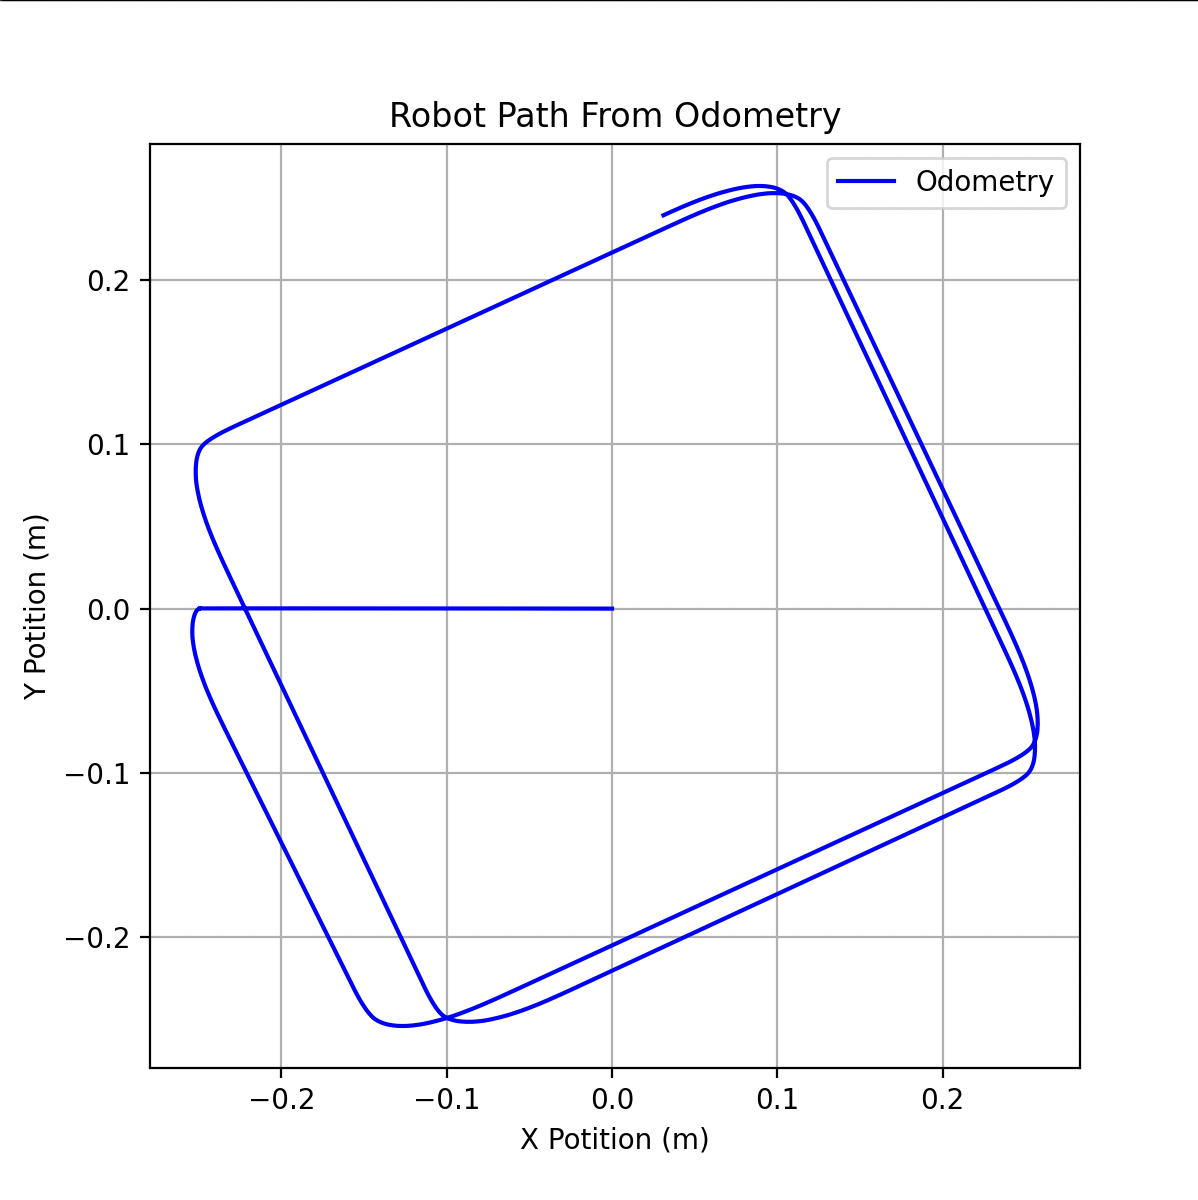
\includegraphics[width=0.5\linewidth]{absolute_potition_graph.png}
    \caption{Grafik Absolute Potition}
    \label{fig:enter-label}
\end{figure}

Lalu, digunakan kode python dibawah untuk mendapat data grafik relative potition sebagai berikut:

\begin{minted}[frame=lines, framesep=2mm, linenos]{python}
# %%
import time
import math
import numpy as np
import matplotlib.pyplot as plt
from datetime import datetime
from coppeliasim_zmqremoteapi_client import RemoteAPIClient

# %%
# 1. Setup Connection
client = RemoteAPIClient()
sim = client.require('sim')

# %%
# 2. Start Simulation
sim.startSimulation()
print("Simulation Started")

# %%
# 3. Simple Test: Post a message to CoppeliaSim status bar
p3dx_RW = sim.getObject("/PioneerP3DX/rightMotor")
p3dx_LW = sim.getObject("/PioneerP3DX/leftMotor")
p3dx = sim.getObject("/PioneerP3DX")

rw = 0.195/2
rb = 0.381/2
d = 0.05
dt = 0.01
x_dot_int = 0.0
y_dot_int = 0.0
gamma_int = 0.0

x_odom = []
y_odom = []
# %%
try:
    # 4. Main Loop (Run for 10 seconds)
    start_time = time.time()
    elapsed_prev = 0.0
    while (time.time() - start_time) < 20:
        
        # --- STUDENT CODE GOES HERE ---
        # Example: Print elapsed time
        elapsed = time.time() - start_time
        print(f"Running... {elapsed:.1f}s", end="\r")

        dt = elapsed - elapsed_prev
        elapsed_prev = elapsed
        
        wr_vel = sim.getJointTargetVelocity(p3dx_RW)
        wl_vel = sim.getJointTargetVelocity(p3dx_LW)

        vx = (wr_vel + wl_vel)*rw/2
        wx = (wr_vel - wl_vel)*rw/rb

        gamma_int = gamma_int + wx*dt

        x_dot = vx * math.cos(gamma_int * 3.14)
        y_dot = vx * math.sin(gamma_int * 3.14)

        x_dot_int = x_dot_int + x_dot*dt
        y_dot_int = y_dot_int + y_dot*dt

        x_odom.append(x_dot_int)
        y_odom.append(y_dot_int)

        #sim.addLog(1, f"Vx:{vx:.1f}m/s, Wx:{wx:.1f}rad/s")
        #sim.addLog(1, f"RW:{wr_vel:.1f}, LW:{wl_vel:.1f}")
        sim.addLog(1, f"x_dot:{x_dot:.1f}m/s, y_dot:{y_dot:.1f}m/s, x_int:{x_dot_int:.1f}m, y_int:{y_dot_int:.1f}m, gamma_int:{gamma_int:.1f}")

finally:
    # 5. Stop Simulation safely
    sim.stopSimulation()
    print("\nSimulation Stopped")

plt.figure(figsize=(6,6))
plt.plot(x_odom, y_odom, 'b-', label='Odometry')
plt.xlabel('X Potition (m)')
plt.ylabel('Y Potition (m)')
plt.title('Robot Path From Odometry')
plt.legend()
plt.grid(True)
plt.show()
\end{minted}

Setelah kode diatas di run, maka nilai joint velocity akan muncul pada terminal CoppeliaSim dan didapatkan grafik relative potition sebagai berikut:

\begin{figure}[H]
    \centering
    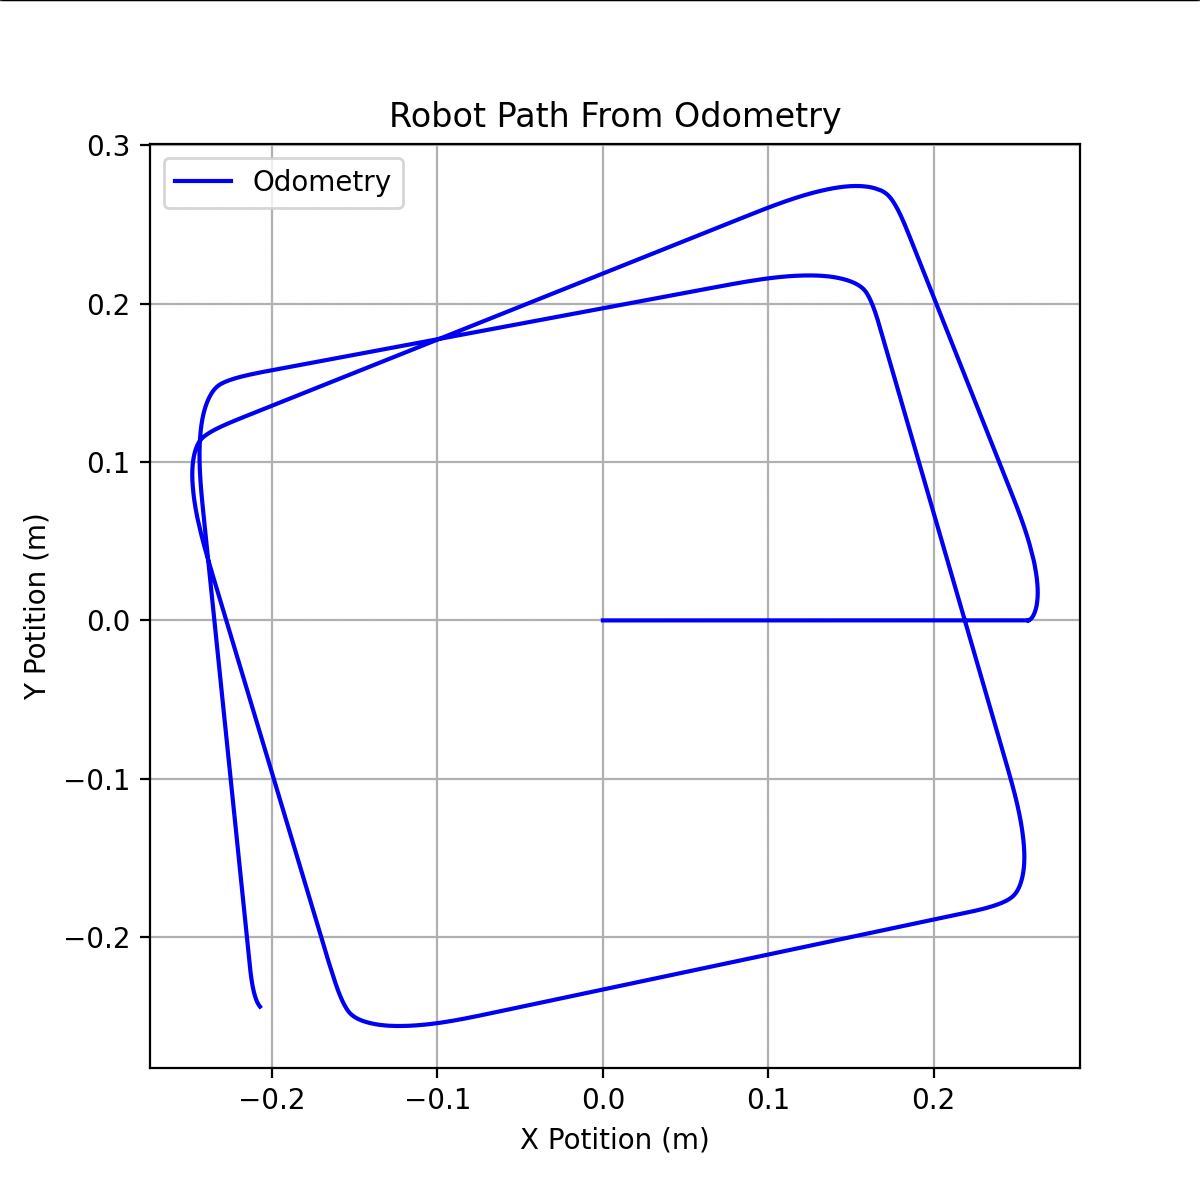
\includegraphics[width=0.5\linewidth]{relative_potition_graph.png}
    \caption{Grafik Relative Potition}
    \label{fig:enter-label}
\end{figure}

Perbedaan antara kedua grafik adalah, absolute potition memberikan posisi real P3DX sesuai dengan sumbunya berada terhadap bidang yang dilewatinya, sedangkan relative potition adalah posisi relatif objek dimana arah depan awal awal objek bergerak di anggap sebagai sumbu x positif.

\end{document}
